\chapter[Figures, Tables, References]{Figures, Tables, and References}
    \label{cha:figures}

\epigraph{%
    The underlying physical laws necessary for the mathematical theory of a large part of physics and the whole of chemistry are thus completely known, and the difficulty is only that the exact application of these laws leads to equations much too complicated to be soluble.}
    {P.~A.~M.~Dirac}

% The following space can be used as a "section abstract" where you summarize the work and its main findings.
%
\noindent This chapter explains the use figures, tables, references and other things important to a PhD thesis typeset with \LaTeX.
%%%%%%%%%%%%%%%%%%%%%%%%%%%%%%%%%%%%%%%%%%%%%%%%%%%%%%%%%%%%%%%%%%%%
% The main content of the chapter begins here
%
\section{Including and referencing figures}
    \label{sec:figures}
    %
    \subsection{A first figure}
        \label{subsec:figures1}
    %
    \Cref{fig:02-PWL} shows how to include a figure.
    %
    Make sure that you understand the float modifiers of the figure environment (i.e., the letters t, b, h, p, and the exclamation mark)
    %
    Always provide a short caption in square brackets, as the long caption is often way too long for the List of Figures.
    %
    Label your figures clearly and systematically, as this will make your life easier once you begin referring to your figures \seeref{subsec:references} .
    %
    \begin{figure}[t]
    \centering
        \includegraphics[width=1.0\textwidth]{I_figures/02_1_PWL.png}
        \caption[Short caption of the PWL condition figure.]{Schematic illustration of the ground-state total energy as a function of electron number. The exact energy is PWL between integer occupations, whereas (semi)local \ac{xc} functionals exhibit a spurious convex curvature. Small misalignments at integer $n$ indicate residual ``endpoint'' errors, as approximate \ac{DFT} is not exact even for integer electron numbers.}
        \label{fig:02-PWL}
    \end{figure}
    %
%%%%%%%%%%%%%%%%%%%%%%%%%%%%%%%%%%%%%%%%%%%%%%%%%%%%%%%%%%%%%%%%%%%%
    \subsection{Another section, another figure}
        \label{subsec:figures2}
    %
    \Cref{fig:02-uimpact} shows another example of a figure; namely one that is scaled down to 90\% of  textwidth.
    %
    Note that the imagefiles are named in a systematic manner (02 for chapter 02=theory and \_2 as it is the second figure shown in this chapter).
    %
    This helps to avoid confusion at later stages of your work, when you have dozens of imagefiles with potentially similar names.
    %
    \begin{figure}[ht]
    \centering
        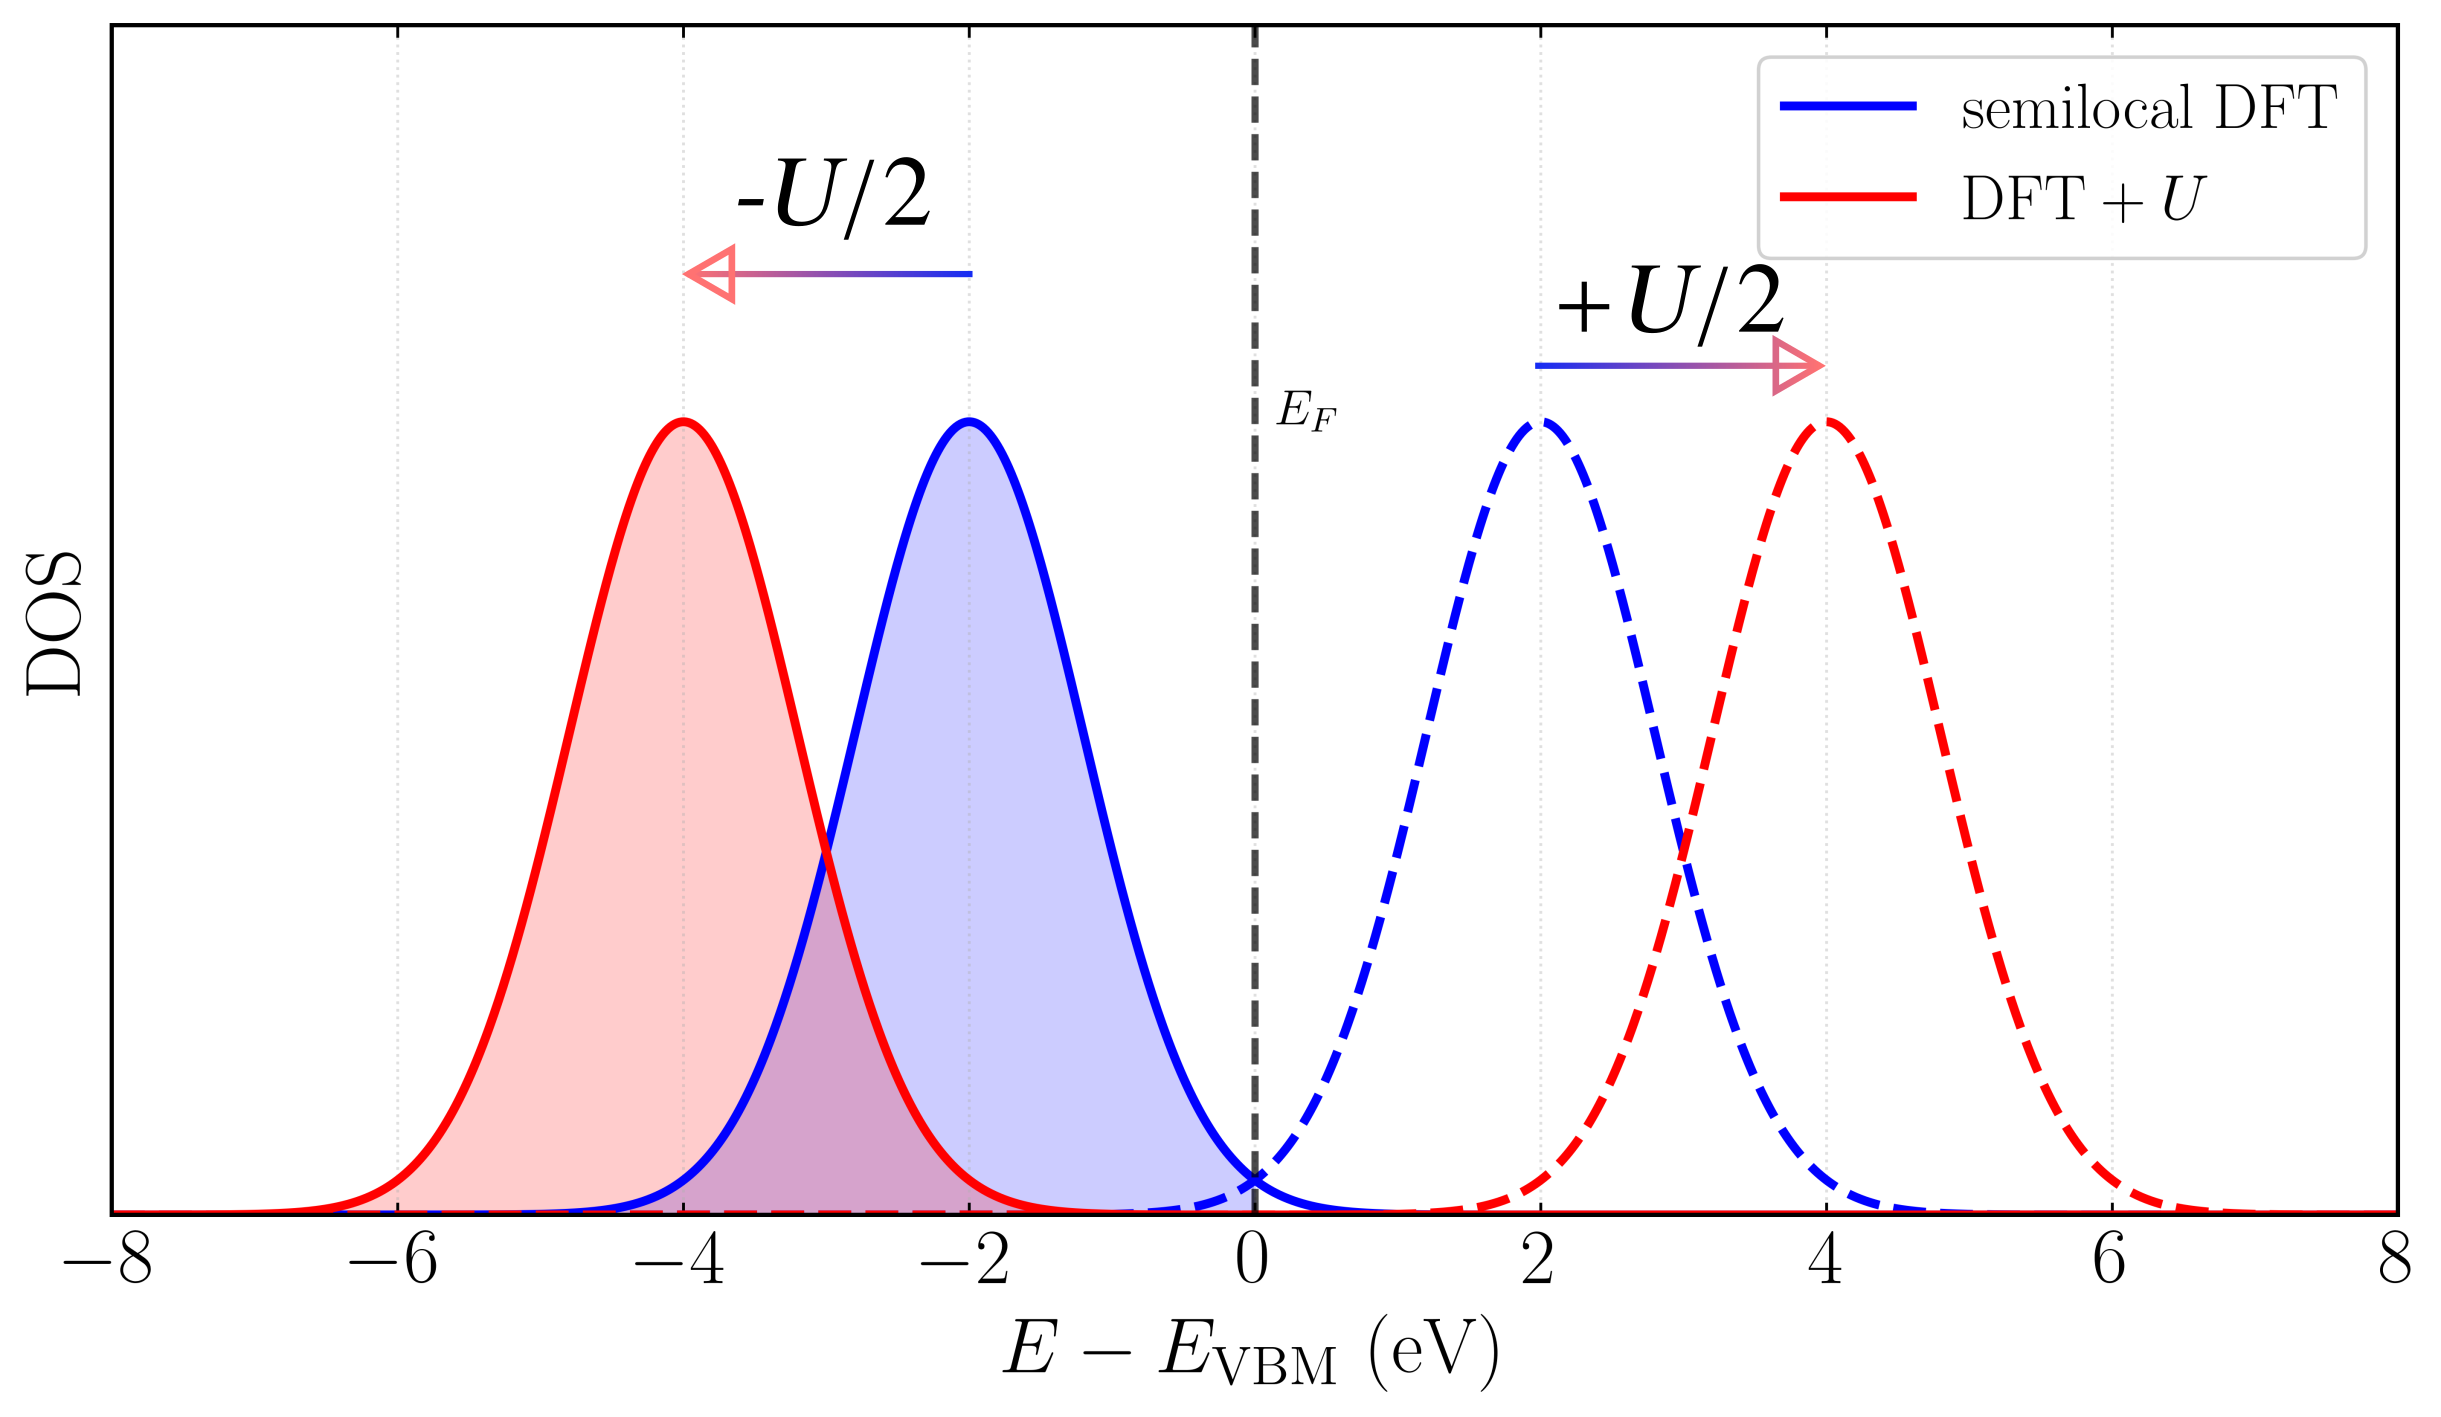
\includegraphics[width=0.9\textwidth]{I_figures/02_2_U-Impact.png}
        \caption[Potential shift due to Hubbard $U$ corrections.]{Impact of an on-site $U$ correction (Dudarev functional) on the energetic levels of the occupied (solid lines) and unoccupied (dashed lines) states of an isolated manifold. The potential of the states is shifted by $\pm U/2$ (here: $U\approx4\,$eV), thus leading to the emergence of a band gap.}
        \label{fig:02-uimpact}
    \end{figure}
    %
%%%%%%%%%%%%%%%%%%%%%%%%%%%%%%%%%%%%%%%%%%%%%%%%%%%%%%%%%%%%%%%%%%%%
\section{Other important things you should know}
      \label{sec:fundamentals}
    %
    \subsection{Internal references}
        \label{subsec:references}
    %
    To refer to chapters, sections, figures, tables, and equations, use the cref command (e.g., \cref{fig:02-PWL}), thanks to which you don't need to put a tilde between the dot after "Fig."., which is required in case you use the classical "ref" command: Fig.~\ref{fig:02-PWL}.
    %
    You can also refer to multiple objects in one command, e.g., \cref{cha:second-results,cha:conclusions}.
    %
    Thanks to the the seeref and cfref macros, \LaTeX automatically renders paraenthesis and puts a "see" or "cf." in front of the reference:  \seeref{cha:conclusions}, \cfref{tab:02-parameters}.
    %
    Make sure you understand the difference between "see" and "cf."!
    %
%%%%%%%%%%%%%%%%%%%%%%%%%%%%%%%%%%%%%%%%%%%%%%%%%%%%%%%%%%%%%%%%%%%%
    \subsection{Citations}
        \label{subsec:citations}
    %
    You have plenty of options to cite works using the natbib package.
    %
    Besides the traditional cite command \cite{andersonMore1972}, you can also make latex print the author's name \textit{together with the citation} (\citet{andersonMore1972}), or without it: \citeauthor{andersonMore1972}.
    %
    Of course, you can also cite multiple references at once: \cite{bornZur1927,giannozziQUANTUM2009,giannozziQuantum2020}.
    %
    If youu want to explicitly refer to a reference, you can print the reference number without the brackets using citenum, e.g., Ref.~\citenum{andersonMore1972}.

    In any case, you should use a consistent naming scheme for your references \textit{from the beginning}, e.g FirstauthornameShorttitleYear.
    %
    Moreover, make sure to avoid unicode symbols incompatible with BibTex (such as the long dash).
    %
    A good and free literature management program is Zotero, which is particularly powerful if you install the (also free) BetterBibTex extension.
    %
%%%%%%%%%%%%%%%%%%%%%%%%%%%%%%%%%%%%%%%%%%%%%%%%%%%%%%%%%%%%%%%%%%%%
    \subsection{Acronyms}
        \label{subsec:acronyms}
    %
    The acronyms package can be very helpful both for you and for the reader to avoid confusion over the use of acronyms.
    %
    Once defined in acronyms.tex, you can invoke an acronym using the ac command: \ac{MAE}.
    %
    Note that when an acronym is invoked for the first time, the package will automatically print the long form and the acronym in parenthesis.
    %
    The second time you refer to the same acronym, like \ac{MAE}, only the short form is shown.

    For plural forms, you can use the acp command, which add an "s" to the last word, unless you defined a different plural form: \acp{MAE}.
    %
    If you want to avoid the long version to be shown, you can tell acronyms that the definitions has already been given through acused.
    %
    \acused{GPU}
    %
    Then, when you invoke the acronym, it will not print the long form: \ac{GPU}.
    %
    However, you can enforce the long form (without the short form) through acl---\acl{GPU}---and vice versa, you can enforce the short form using acs: \acs{GPU}.
    %
%%%%%%%%%%%%%%%%%%%%%%%%%%%%%%%%%%%%%%%%%%%%%%%%%%%%%%%%%%%%%%%%%%%%
    \subsection{Tables}
        \label{subsec:tables}
    %
    \Cref{tab:02-parameters} shows an example of a table environment.
    %
    Always remember that tables have titles (above them) rather than captions (below the object).
    %
    A good tool for creating tables in Latex (e.g., with the good-looking booktabs style) can be found at \url{https://tablesgenerator.com/}.
    %
    \begin{table}[ht]
        \centering
        \setlength{\tabcolsep}{4pt}
        \renewcommand{\arraystretch}{1.6} 
        \caption[Short caption of the \ce{AUO4} Hubbard U table.]{Self-consistent Hubbard $U$ parameters obtained from LR-cDFT for three setups (one shell-averaged plus two orbital-resolved) with differently defined Hubbard manifolds. The values in parentheses are those derived and applied by \citet{wardaGetting2025}.}
        %
        \begin{tabular}{c c c c c}
            \arrayrulecolor{black}\hline
              System & \multicolumn{4}{c}{$U$ (eV)} \\  \hline
            \rowcolor{gray!10}[6pt] Shell-averaged
               & A-$3d$ & U-$5f$ & O1-$2p$ & O2-$2p$ \\ 
        
               \ce{\beta-NiUO4} & 7.03 (6.6) & 3.65 (2.6) & 7.56 & 7.97 \\ 
               \ce{MnUO4} & 7.34 (4.4) & 3.92 (2.7) & 7.45 & 7.82 \\ 
               \ce{CoUO4} & 6.19 (5.2) & 3.77 (2.7) & 7.54 & 7.94\\ 
        
            \rowcolor{gray!10}[6pt] Setup (1)
               & A-$3d$ & U-${5f}_{\nu_1-\nu_4}$ & O1-$2p$ & O2-$2p$ \\ 
        
               \ce{\beta-NiUO4} & 7.03 & 1.37 & 7.59 & 7.97 \\ 
               \ce{MnUO4} & 7.17 & 1.38 & 7.49 & 7.87 \\ 
               \ce{CoUO4} & 6.20 & 1.36 & 7.56 & 7.94\\ 
               
            \rowcolor{gray!10}[6pt] Setup (2)
               & A-${\widetilde{t_{2g}}}$ & U-${5f}_{\nu_1-\nu_4}$ & O1-$2p$ & O2-$2p$ \\ 
               
               \ce{\beta-NiUO4} & 7.40 & 1.33 & 7.50 & 7.78 \\ 
               \ce{MnUO4} & 1.27 & 0.93 & 7.40 & 7.74 \\ 
               \ce{CoUO4} & 2.33 & 1.22 & 7.47 & 7.77 \\ 
            \arrayrulecolor{black}\hline       
        \end{tabular}
        \label{tab:02-parameters}
    \end{table}
    %
%%%%%%%%%%%%%%%%%%%%%%%%%%%%%%%%%%%%%%%%%%%%%%%%%%%%%%%%%%%%%%%%%%%%
    \subsection{Equations}
        \label{subsec:eqs}
    %
    Finally, you can typeset equations using the "equation", "gathered" and "align" environments:
    %
    \begin{equation}
     \frac{\partial}{\partial\vec{R}^K}\left\langle \phi^I_m | \psi^\sigma_{\vec{k}v} \right\rangle   \,.
     \label{eq:2-hub-force}
    \end{equation}
    %
    Never forget that equations should also follow punctuation rules, thus ending either with a full stop or with a comma, like in
    \begin{equation}
        \begin{gathered}
        \frac{\partial E_\mathrm{Hub}}{\partial \vec{R}^K} = \sum_{I}\sum_{\sigma,m,m'} \frac{\partial E_\mathrm{Hub}}{\partial n^{I\sigma}_{mm'}} \frac{\partial n^{I\sigma}_{mm'}}{\partial\vec{R}^K} \\
        = \sum_{I}\sum_{\sigma,m,m'} U^I\left( \frac{\delta_{mm'}}{2}-  n^{I\sigma}_{mm'} \right) \frac{\partial n^{I\sigma}_{m'm}}{\partial\vec{R}^K} \, ,
        \end{gathered}
        \label{eq:2-hub-force2}
    \end{equation}
    %
    which represents a complicated force term.
    %
    Again, use a reasonable labeling scheme so that you can easily refer to your equation, e.g. \cref{eq:2-hub-force}, later on.